\section{Prototyping}

Nachdem ein Gesamtkonzept geplant wurde, wird nun möglichst viel Prototyping durchgeführt. Das Ziel ist es, zu testen, ob das ermittelte Konzept funktionieren könnte oder ob es überarbeitet werden muss. So kann mit den Risiken, die im vorhergehenden Kapitel ermittelt wurden, besser umgegangen werden.

\subsection{...}

\subsection{Kürzester Weg finden}

Da es nur 8 Knoten im Graph gibt, wurde von Anfang an vermutet, dass die Geschwindigkeit des Algorithmus vernachlässigt werden kann.

Um zu überprüfen, dass diese These stimmt, wurde ein traditioneller Dijkstra Algorithmus in Python implementiert. Dabei wurde von einem Knoten den kürzesten Weg zu allen anderen Knoten im vorgegebenen Graphen berechnet. währendessen wurde die Zeit für die Berechnungen gestoppt. Um Hardware Einflüsse zu minimieren, wurde dieses Skript auch auf einem Single-Board Computer, namentlich einem Raspberry Pi 4 (4GB) ausgeführt, und einige male wiederholt. Was uns zu nachfolgender Ausgabe und Kenntnissen bringt:

\begin{verbatim}
Shortest distance from E to A is 18 via path: E -> G -> A
Shortest distance from E to B is 22 via path: E -> G -> H -> B
Shortest distance from E to C is 20 via path: E -> D -> C
Shortest distance from E to D is 10 via path: E -> D
Shortest distance from E to E is 0 via path: E
Shortest distance from E to F is 10 via path: E -> F
Shortest distance from E to G is 6 via path: E -> G
Shortest distance from E to H is 12 via path: E -> G -> H
This calculation took about 0.128ms
\end{verbatim}

Das Skript wurde in einem Github Gist veröffentlicht und ist unter folgendem Link aufrufbar: \url{https://gist.github.com/dimschlukas/2632116f913b1e10eea9be40e62b2630}

Um den kürzesten Pfad achtmal zu berechnen, wurden etwa 0,128 ms benötigt, was ausreichend schnell ist. Aufgrund dieses Tests wurde entschieden, einen selbst implementierten, einfachen Dijkstra-Algorithmus zu verwenden, da es wichtig ist, dass der Algorithmus möglichst leichtgewichtig ist, da nur begrenzte Rechenleistung und Speicher zur Verfügung stehen.

\subsection{Bilderkennung}

\subsubsection{Spiegelung}

spiegelt stark, vor allem Problem, um Knoten zu erkennen; Bilder entspiegeln: Lichtverhaeltnisse, Polfilter oder Nachbearbeitung.\cite{avoid-reflection}

\subsubsection{YOLOv11}

Auf Roboflow\footnote{https://roboflow.com/} Bilder labeled: (Als erstes mit Linie versucht, das geht nicht ev Bild) 

TODO BILD

Mihilfe eines Jupyter skripts Yolo Model trainieren mit 10 Epochs, Confusion Matrix und Bilder:

\begin{figure}[H]
\centering
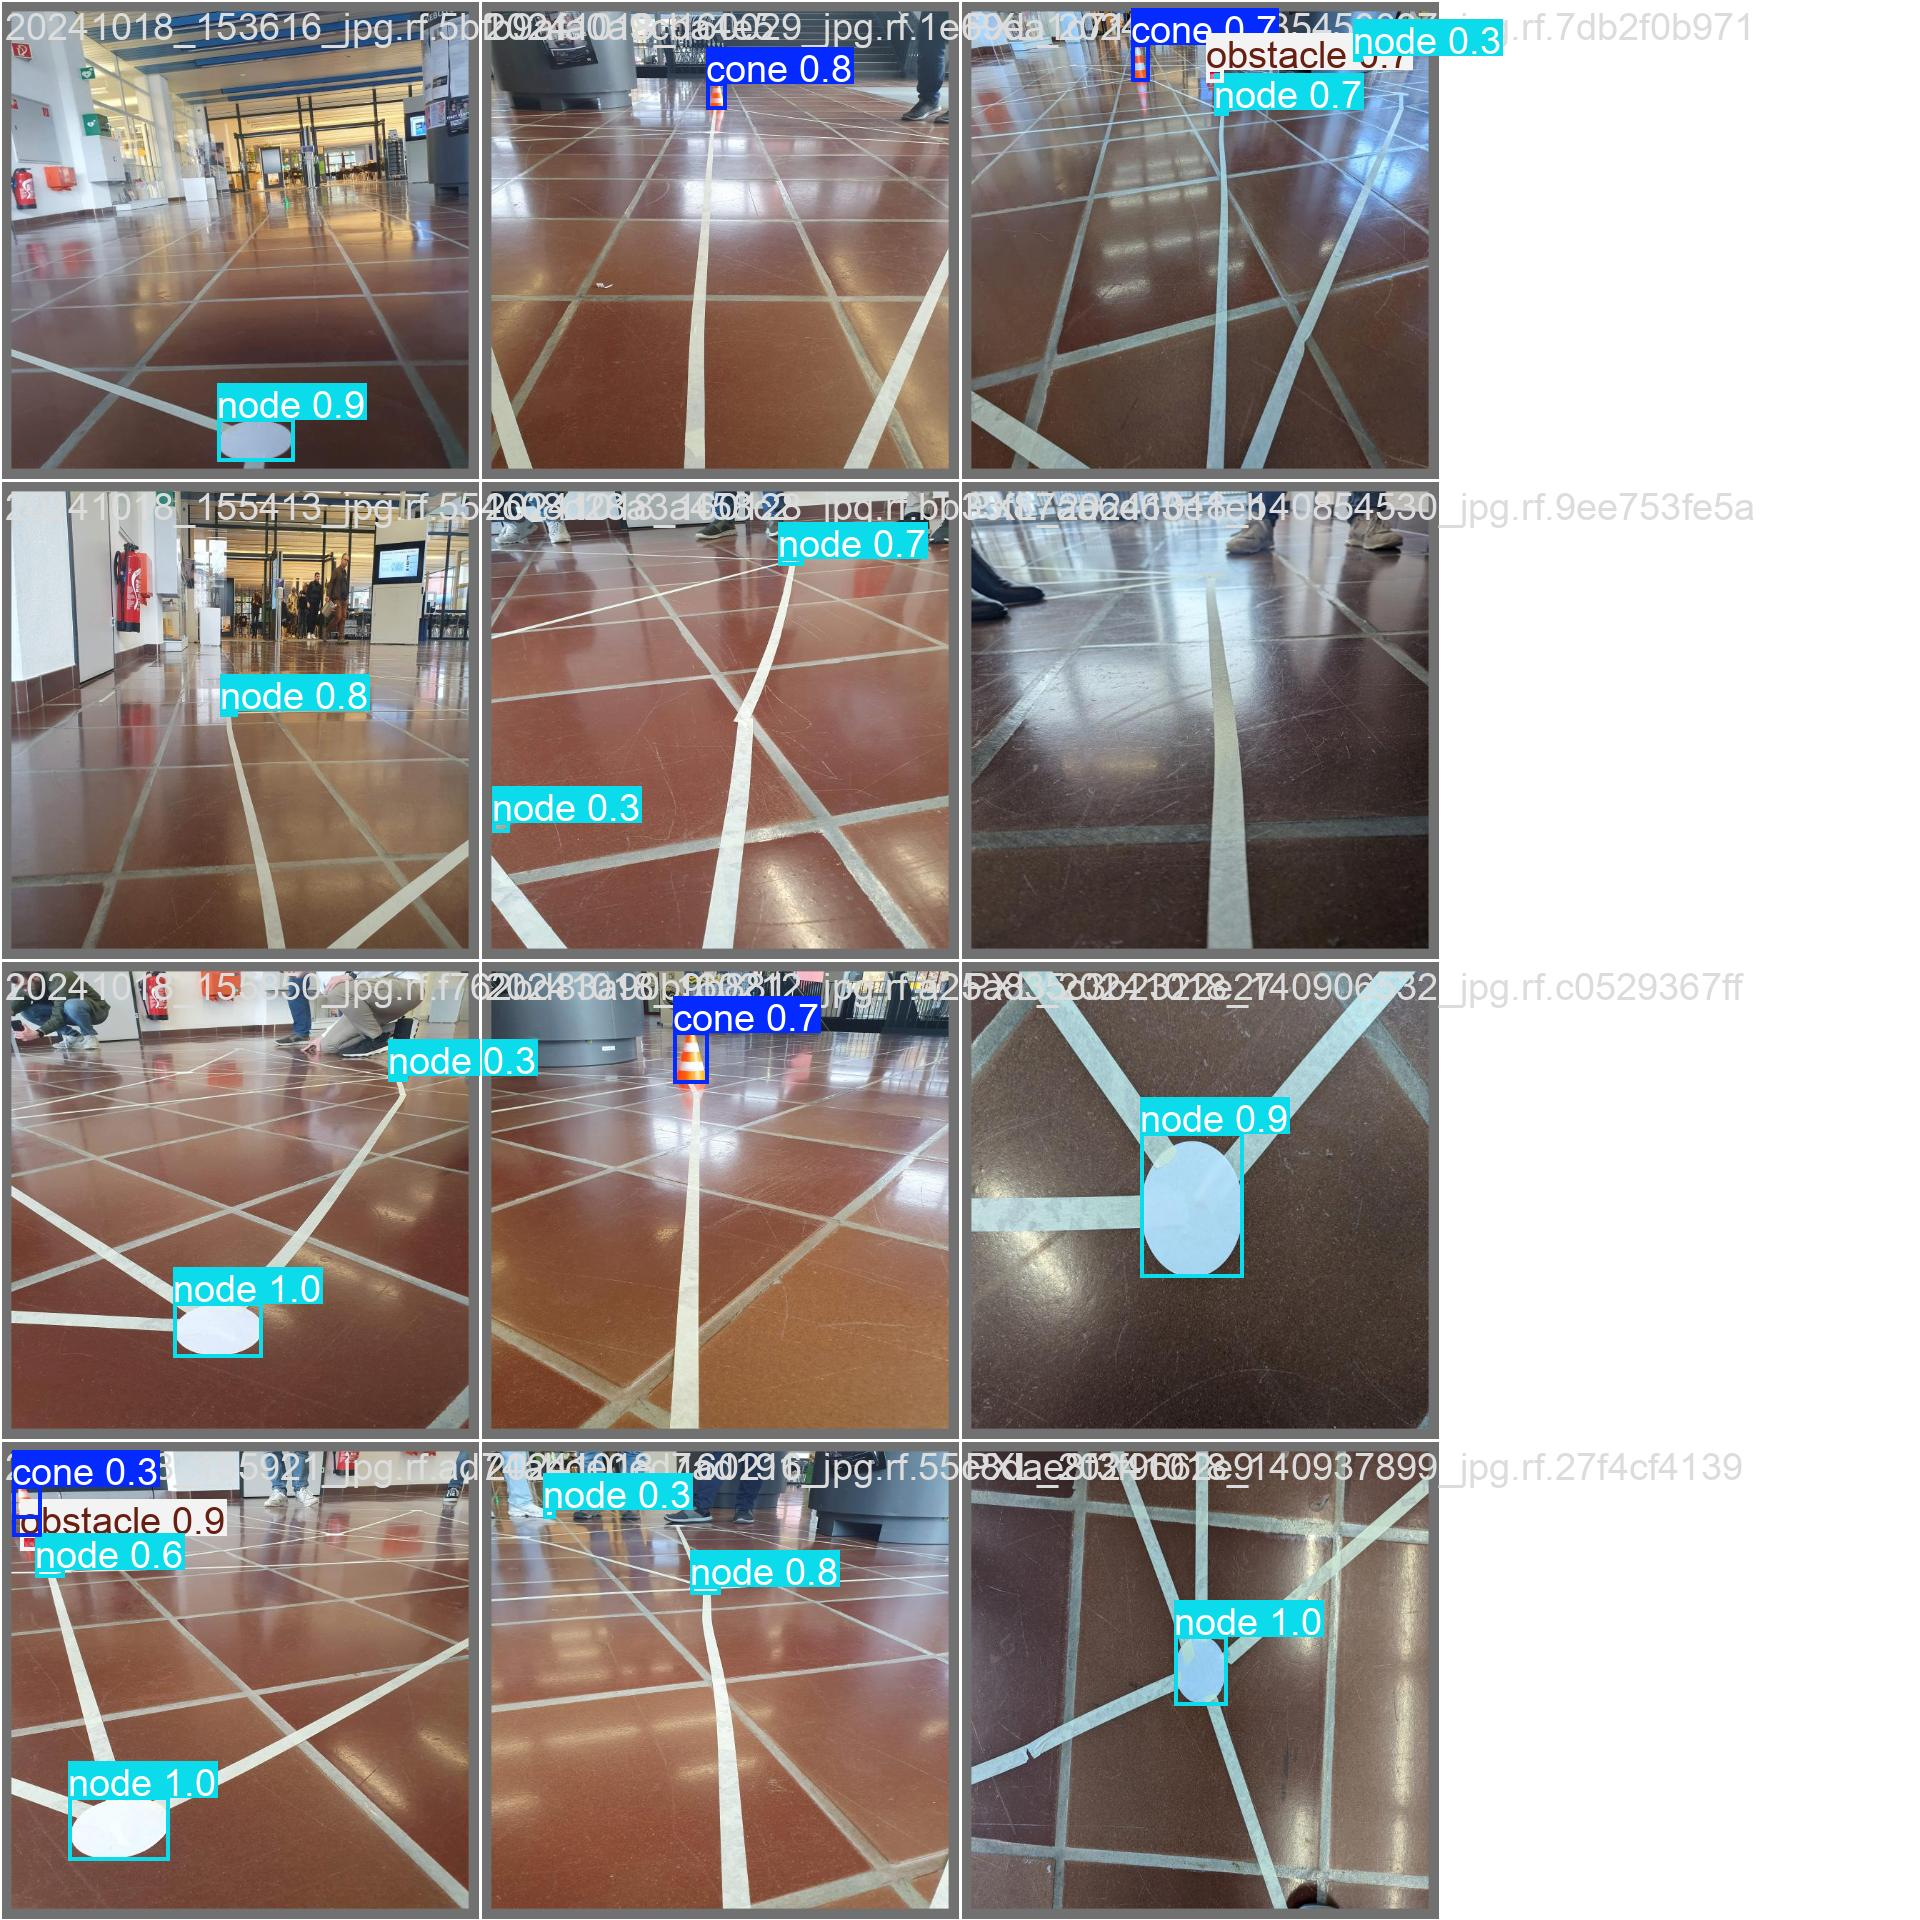
\includegraphics[width=\textwidth -30mm]{assets/informatik-prototyp/yolo/recognized-images.jpeg}
\caption{YOLOv11 Bilderkennung}
\label{fig:img-recognition-yolo}
\end{figure}

-> Yolo kann relativ gut erkennen, vor allem wenn Knoten nicht zu weit weg sind

\subsection{Simulator}

TODO: eigenes File?

Das Erarbeiten des Konzeptes des Simulators, der Implementierung und des Gebrauchs wird in diesem Kapitel festgehalten.

Nach der Nutzwertanalyse war das grundlegende Konzept klar und es konnte mit der Implementierung begonnen werden.

- GitHub, Issues sammeln, Festlegen Git ettiquete (aka MRs)

- Struktur mit Klassen (ERD?): Robot, Reader, Calculator, GUI

- Roboter liest Graph, ueberprueft Nodes und Barrieren

- Calculator holt kürzester Weg, Roboter geht zu nächsten Node

- Poetry

- Die einzelnen Kanten werden identifiziert mit Sortierung

- GUI Roboter bewegt sich
